%!TEX root = ../username.tex
\chapter{Realtime Audio Programming}
\hspace*{-0.12cm}This chapter will consider the theory behind audio programming and the different principles that are followed to create a functional program.
\section{Sound As A Discrete Signal}
Sound is a physical phenomenon. Vibrations travel though a medium such as air to create waves and differences in pressure which travel at the the speed of sound (roughly 343 m/s). Naturally, representing this in a digital setting involves simplifying the physical nature of sound waves into an easily digestible format.

Consider Figure 3.1:

\begin{figure}[h] % [h] used to prevent {figure} from doing weird positioning
\begin{center}
	\fbox{
	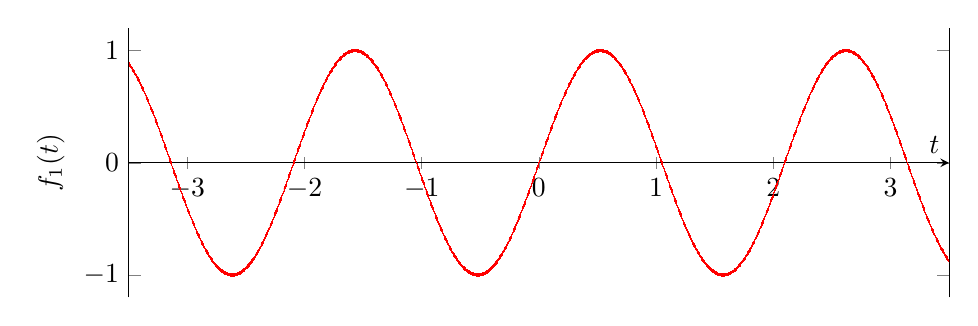
\begin{tikzpicture}
		\begin{axis} [
			axis x line = middle, % The x axis should go through the origin
			xlabel = \(t\),
			ylabel = {\(f_1(t)\)},
			height = 5cm,
			width = 12cm
			]

			\addplot [
			jump mark mid,
			domain = -3.5:3.5,
			samples = 1000,
			very thick, red
			] {(sin(deg(3 * x)))};

		\end{axis}
	\end{tikzpicture}}
	\caption{A graph of the sine wave \(f_1(t) = sin(3t)\).}
\end{center}
\end{figure}

This is a representation of a sinusoid under the time domain. This tone is often described as ``pure'' for its lack of overtones. One can represent this digitally by taking measurements of the function \(f_1(t)\) at regular points in time, each known as a \textit{sample}. By convention, samples are in the range (-1,1). By graphing each sample into the function \(f_2(t)\), one can create a digital version of this analog signal.

\begin{figure}[h] % [h] used to prevent {figure} from doing weird positioning
	\begin{center}
		\fbox{
		\begin{tikzpicture}
			\begin{axis} [
				axis x line = middle, % The x axis should go through the origin
				xlabel = \(t\),
				ylabel = {\(f_2(t)\)},
				height = 5cm,
				width = 12cm
				]

				\addplot+ [
				ycomb,
				mark = text,
				text mark = , % so jank
				domain = -3.5:3.5,
				samples = 40,
				red
				] {(sin(deg(3 * x)))};

			\end{axis}
		\end{tikzpicture}
		}
		\caption{A discrete graph of the sine wave \(f_2(t) = sin(3t)\) taken with 40 samples.}
	\end{center}
\end{figure}

This is a discrete representation of our original graph \(f_1(t) = sin(3t)\).

\section{The Realtime Programming Bus Schedule}
[] Unlike a music player, our program has to follow the set schedule requested by the audio driver of a device [].
\section{The Golden Rules}
\section{Software Available}
